\documentclass[border=1cm]{standalone}

\usepackage{tikz}
\usetikzlibrary{3d}

\begin{document}
    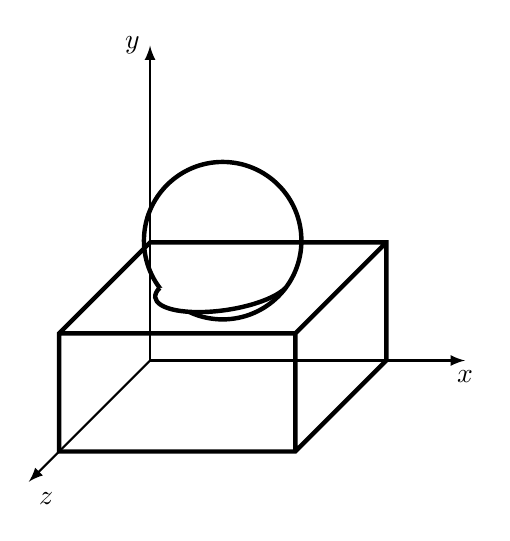
\begin{tikzpicture}[scale=0.1]
        \coordinate (A) at (30,0,30);
        \coordinate (B) at (30,0,0);
        \coordinate (C) at (0,0,0);
        \coordinate (D) at (0,0,30);
        \coordinate (E) at (30,15,30);
        \coordinate (F) at (30,15,0);
        \coordinate (G) at (0,15,0);
        \coordinate (H) at (0,15,30);

        \draw[->,>=latex,thick](0,0)--(40,0)node[below]{$x$};
        \draw[->,>=latex,thick](0,0)--(0,40)node[left]{$y$};
        \draw[->,>=latex,thick](0,0)--(0,0,40)node[below right]{$z$};

        \draw[ultra thick] (D)--(A)--(B)--(F)--(G)--(H)--cycle (H)--(E)--(F) (E)--(A);
        \begin{scope}[canvas is xy plane at z=15]
            \draw[ultra thick] (15,21) circle (10cm);
        \end{scope}
        
        \begin{scope}[canvas is xz plane at y=15]
            \draw[ultra thick, fill=white] (15+8,15) arc [start angle=0, end angle=180, radius=8];
        \end{scope}

    \end{tikzpicture}
\end{document}